\documentclass[11pt]{article}
\usepackage{times}
\usepackage[cm]{fullpage}
\usepackage{amsmath,amssymb}
\usepackage{booktabs}
\usepackage{tabularx}
\newcolumntype{Y}{>{\raggedright\arraybackslash}X}
\usepackage{enumitem}
\usepackage{microtype}
\usepackage{hyperref}
\usepackage{tikz}
\usetikzlibrary{arrows.meta,positioning,fit,backgrounds,calc,shapes.geometric}
\hypersetup{hidelinks}

\definecolor{primitivecol}{RGB}{85,85,85}
\definecolor{optioncol}{RGB}{183,83,42}
\definecolor{landmarkcol}{RGB}{42,104,155}
\definecolor{pathcol}{RGB}{190,55,55}
\definecolor{loopcol}{RGB}{216,140,30}
\definecolor{decoycol}{RGB}{150,90,160}

\tikzset{
  task state/.style={circle,draw,minimum size=8mm,inner sep=0pt,font=\small\bfseries},
  task landmark/.style={task state,fill=landmarkcol!22,draw=landmarkcol,line width=1pt},
  task decoy/.style={task state,draw=decoycol,line width=1pt,densely dotted},
  gridedge/.style={-{Stealth[length=3pt]},draw=black!28,line width=0.8pt},
  loopedge/.style={-{Stealth[length=4pt]},draw=loopcol,line width=1.4pt,densely dashed},
  pathedge/.style={-{Stealth[length=5pt]},draw=pathcol,line width=2.3pt},
  macroL/.style={-{Stealth[length=4pt]},draw=landmarkcol,line width=1.5pt},
  macroG/.style={-{Stealth[length=4pt]},draw=optioncol,line width=1.5pt}
}

\title{A Three-Landmark Option Agent and Its Closest Action-Chunk Twin\\
\large Analysis 9: A worked instance on a grid-with-loop task, and how to tell them apart}
\author{}
\date{6 June 2026}

\begin{document}
\maketitle

\begin{abstract}
This note instantiates the Analysis-7/8 framework on one concrete task: a $3\times3$
transition grid augmented with a one-way directed loop. We build a landmark-option agent
whose representation is three optimal landmarks and the directed relations among them,
and show exactly how it generates a plan and searches. We then construct the
\emph{closest} action-chunk (temporal-abstraction) agent: a grammar with one reusable
action string that reproduces the landmark agent's modal trajectory. On the canonical
start--goal trial the two agents are behaviourally identical. We then identify the trials
and measures on which they diverge, compare their induced cognitive maps, and pose the
system-identification questions and recovery tests needed to decide which agent generated
a given behavioural record. The recovery section states questions and proposed tests only;
it does not run them.
\end{abstract}

\section{The instance task}

\subsection{Primitive graph $\mathcal K_0$}

States are nine cells of a $3\times3$ grid,
\[
\mathcal S=\{1,\dots,9\},\qquad
\begin{smallmatrix}
1&2&3\\[1pt]4&5&6\\[1pt]7&8&9
\end{smallmatrix}.
\]
The primitive action set is $\mathcal A=\{\mathsf R,\mathsf D,\mathsf X\}$. The local
moves $\mathsf R$ (right) and $\mathsf D$ (down) give the usual forward grid edges. The
third action $\mathsf X$ is a one-way \emph{express} move, available only at the four
mid-edge ``loop-tail'' states $\{2,4,6,8\}$, that advances one stop clockwise around the
centre:
\[
2\xrightarrow{\mathsf X}6,\quad
6\xrightarrow{\mathsf X}8,\quad
8\xrightarrow{\mathsf X}4,\quad
4\xrightarrow{\mathsf X}2 .
\]
These four edges form a single directed loop $\Lambda$ (Fig.~\ref{fig:task}). Every edge
costs one step. The loop makes $\mathcal K_0$ cyclic, so the grid distance and the
loop-using distance differ: with start $s_0=1$ and goal $s_\star=9$,
\[
d_{\mathrm{grid}}(1,9)=4,
\qquad
d_{\mathrm{loop}}(1,9)=3
\quad\text{via}\quad
1\xrightarrow{\mathsf R}2\xrightarrow{\mathsf X}6\xrightarrow{\mathsf D}9 .
\]
The express edge $2\xrightarrow{\mathsf X}6$ is a genuine shortcut: each $\Lambda$-edge
replaces a two-step grid detour. The grid alone admits $\mu_{\mathrm{sp}}(1,9)=6$
shortest paths of length $4$; the loop adds shorter and qualitatively different routes.

\begin{figure}[htbp]
\centering
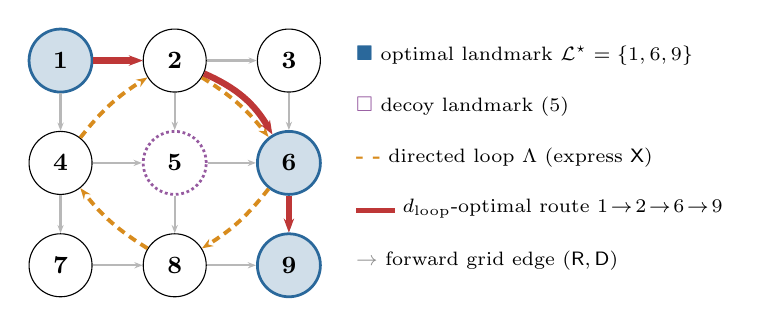
\begin{tikzpicture}[x=1.45cm,y=1.3cm]
  \node[task landmark] (s1) at (0,2) {1};
  \node[task state]    (s2) at (1,2) {2};
  \node[task state]    (s3) at (2,2) {3};
  \node[task state]    (s4) at (0,1) {4};
  \node[task decoy]    (s5) at (1,1) {5};
  \node[task landmark] (s6) at (2,1) {6};
  \node[task state]    (s7) at (0,0) {7};
  \node[task state]    (s8) at (1,0) {8};
  \node[task landmark] (s9) at (2,0) {9};

  % forward grid edges
  \foreach \a/\b in {s1/s2,s2/s3,s4/s5,s5/s6,s7/s8,s8/s9}{\draw[gridedge] (\a)--(\b);}
  \foreach \a/\b in {s1/s4,s4/s7,s2/s5,s5/s8,s3/s6,s6/s9}{\draw[gridedge] (\a)--(\b);}

  % directed loop Lambda (drawn slightly bent to read as a cycle)
  \draw[loopedge] (s2) to[bend left=10] (s6);
  \draw[loopedge] (s6) to[bend left=10] (s8);
  \draw[loopedge] (s8) to[bend left=10] (s4);
  \draw[loopedge] (s4) to[bend left=10] (s2);

  % express optimal route 1-2-6-9
  \draw[pathedge] (s1) to[bend left=0] (s2);
  \draw[pathedge] (s2) to[bend left=18] (s6);
  \draw[pathedge] (s6) -- (s9);

  \node[anchor=west,font=\scriptsize] at (2.5,2.05)
    {\textcolor{landmarkcol}{$\blacksquare$}\ optimal landmark $\mathcal L^\star=\{1,6,9\}$};
  \node[anchor=west,font=\scriptsize] at (2.5,1.55)
    {\textcolor{decoycol}{$\square$}\ decoy landmark (5)};
  \node[anchor=west,font=\scriptsize] at (2.5,1.05)
    {\textcolor{loopcol}{\textbf{- -}}\ directed loop $\Lambda$ (express $\mathsf X$)};
  \node[anchor=west,font=\scriptsize] at (2.5,0.55)
    {\textcolor{pathcol}{\rule{5mm}{1.6pt}}\ $d_{\mathrm{loop}}$-optimal route $1\!\to\!2\!\to\!6\!\to\!9$};
  \node[anchor=west,font=\scriptsize] at (2.5,0.05)
    {\textcolor{black!45}{$\rightarrow$}\ forward grid edge ($\mathsf R,\mathsf D$)};
\end{tikzpicture}
\caption{The instance task $\mathcal K_0$: a $3\times3$ grid of forward $\mathsf R/\mathsf D$
edges plus a one-way directed loop $\Lambda$ realized by the express action $\mathsf X$ at
the four mid-edge states. Start $1$, goal $9$. The three optimal landmarks are the start
anchor $1$, the express hub $6$, and the goal anchor $9$; the centre $5$ is a strong
\emph{decoy} that is optimal under the grid alone but is bypassed once the loop exists.}
\label{fig:task}
\end{figure}

\subsection{Why three landmarks, and which three}

Landmarks are scored by task-weighted salience (betweenness / bottleneck coverage under
the start--goal distribution); this ranking only \emph{initializes} the candidate set and
is not itself an agent. Under a corner-to-corner task family the optimal three are
\[
\mathcal L^\star=\{1,6,9\}:
\]
$1$ and $9$ are the boundary anchors, and $6$ is the highest-betweenness interior node
\emph{because} the express edge $2\!\to\!6$ funnels optimal routes onto $6$ and then onto
$6\!\to\!9$. The geometric centre $5$ is the natural decoy: it lies on grid-optimal
diagonals but not on the loop-optimal route, so an agent that anchors on $5$ behaves
differently from one that anchors on $6$. This decoy is deliberate; it gives the
identification analysis (Sec.~\ref{sec:recover}) something nontrivial to resolve.

\subsection{Matched cover stories}

The same $\mathcal K_0$ is presented through two surfaces. In \emph{navigation}, states are
locations, $\mathsf R/\mathsf D$ are moves, and $\mathsf X$ is a one-way corridor. In
\emph{crafting}, states are object configurations, $\mathsf R/\mathsf D$ are operations,
and $\mathsf X$ is a catalyst step that jumps between configurations. The latent graph,
landmarks, and loop are identical; only the labels differ.

\section{The landmark-option agent}

\subsection{Representation and induced map}

The agent stores three landmarks and their directed connectivity,
\[
\mathcal R_{\mathrm{landmark}}=(\mathcal L,\mathcal E^{\mathcal L}),
\qquad
\mathcal L=\{1,6,9\},
\qquad
\mathcal E^{\mathcal L}=\{(1,6),(6,9),(1,9)\}.
\]
Following Analysis~7, the induced cognitive map is the \emph{hybrid} graph
$\mathcal K_{\mathrm{landmark}}=F_{\mathrm{landmark}}(\mathcal K_0,\mathcal R_{\mathrm{landmark}})$ with
\[
\mathcal V_{\mathrm{landmark}}=\mathcal S,
\qquad
\mathcal E_{\mathrm{landmark}}
=\mathcal E_0\cup
\{(\ell_i,(\ell_i,\ell_j),\ell_j):(\ell_i,\ell_j)\in\mathcal E^{\mathcal L}\}.
\]
The primitive map is retained, and the landmark edges add optional directed shortcuts. The
token support is
\[
\mathcal Z_{\mathrm{landmark}}(x)
=\mathcal A(x)\cup
\{(\ell_i,\ell_j)\in\mathcal E^{\mathcal L}:\ell_i=x\},
\]
so a landmark option becomes available \emph{only at a landmark}; everywhere else the
agent uses primitive $\mathsf R/\mathsf D$ (and $\mathsf X$ at loop tails). At state $1$,
\[
\mathcal Z_{\mathrm{landmark}}(1)
=\{\mathsf R,\mathsf D\}\cup\{(1,6),(1,9)\}.
\]

\subsection{How a plan is generated: search}

All families share one probabilistic heuristic-search kernel over the induced map. For
$z\in\mathcal Z_M(x)$ leading to $x'$,
\[
p_{\mathrm S}(z\mid x,s_\star,\mathcal K_M,\theta_{\mathrm S})
=\frac{\exp\{S_M(x,z,s_\star;\omega_M,\theta_{\mathrm S})\}}
{\sum_{z'\in\mathcal Z_M(x)}\exp\{S_M(x,z',s_\star;\omega_M,\theta_{\mathrm S})\}},
\]
with a goal-directed score, e.g.
$S_M(x,z,s_\star)=-\beta\,\bigl[c(z)+\widehat d_{M}(x',s_\star)\bigr]$,
where $c(z)$ is the token's expected step cost, $\widehat d_M$ is the search heuristic
(estimated remaining cost on $\mathcal K_M$), and $\beta=\theta_{\mathrm S}$ is the search
inverse-temperature. Search budget and score form are held identical across families; only
the available tokens and their endpoints change.

\paragraph{Worked trace, trial $1\to9$.}
At the landmark $1$, the option $(1,9)$ points an admissible heuristic straight at the
goal and compresses the remaining problem to a single decision, so it carries the highest
score; the agent selects $z_{n,1}=(1,9)$ (it could instead select $(1,6)$ and re-plan at
$6$; both give the same observable route). A landmark option specifies \emph{endpoints,
not a motor program}. Execution unfolds through primitive states under a target-directed
kernel
\[
p_{\mathrm E}(a\mid s,z=(\ell_i,\ell_j),\theta_{\mathrm E},\mathcal K_0)
\propto
\exp\{-\eta\,d_{\mathcal K_0}(s'(s,a),\ell_j)\},
\]
which at each step prefers the action that most reduces primitive distance to the target
landmark. From $1$ toward $9$ this descends through the express hub, emitting
\[
1\xrightarrow{\mathsf R}2\xrightarrow{\mathsf X}6\xrightarrow{\mathsf D}9 ,
\]
the $d_{\mathrm{loop}}$-optimal route. Because the kernel scores actions by remaining
distance, \emph{the same token $(1,9)$ can emit several different routes}: if the express
edge is unattractive or unavailable, the agent still reaches $9$ via $1\to2\to5\to6\to9$
or $1\to4\to5\to8\to9$. The endpoint is fixed; the path is flexible. Search expansions are
few, because each landmark option collapses a multi-step segment into one decision.

\section{The closest action-chunk twin}

\subsection{Construction}

We now build the action-chunk agent that most nearly reproduces the landmark agent's modal
behaviour. Its representation is a grammar with one reusable action string that encodes the
express on-ramp,
\[
\mathcal R_{\mathrm{option}}=\mathcal G,
\qquad
\mathcal G=\{\,g_\star=(\mathsf R,\mathsf X)\,\},
\]
optionally augmented by $g_2=(\mathsf R,\mathsf X,\mathsf D)$ for the full route. Applying
$\mathcal G$ to $\mathcal K_0$ adds a labelled macro-edge wherever the string is
executable:
\[
\mathcal E_{\mathrm{option}}
=\mathcal E_0\cup\{e_{g}(x)=(x,g,f(x,g)):x\in\mathcal S,\ g\in\mathcal G(x)\},
\qquad
\mathcal Z_{\mathrm{option}}(x)=\mathcal A(x)\cup\mathcal G(x).
\]
The string $g_\star=(\mathsf R,\mathsf X)$ is executable only where an $\mathsf R$ lands on
a loop tail, i.e. from $\{1,5,7\}$, giving the macro-edges
\[
1\xrightarrow{g_\star}6,\qquad
5\xrightarrow{g_\star}8,\qquad
7\xrightarrow{g_\star}4 .
\]

\paragraph{Worked trace, trial $1\to9$.}
At $1$ the chunk token $g_\star$ has high search score (it advances two steps toward the
goal in one decision), so the agent selects $z_{n,1}=g_\star$. Its emission
$p_{\mathrm E}(\sigma\mid g_\star)$ concentrates on the fixed string $(\mathsf R,\mathsf X)$,
producing $1\to2\to6$; the agent then takes primitive $\mathsf D$ to reach $9$:
\[
\underbrace{1\xrightarrow{\mathsf R}2\xrightarrow{\mathsf X}6}_{g_\star=(\mathsf R,\mathsf X)}
\xrightarrow{\mathsf D}9 .
\]
On this trial the chunk twin and the landmark agent emit \emph{the same primitive
trajectory}. The difference is hidden in what the token means: $g_\star$ is the action
string $(\mathsf R,\mathsf X)$, not the endpoint pair $(1,6)$.

\section{One observed path, three latent explanations}

Table~\ref{tab:explain} writes the same observed trajectory under each family's
segmentation, exactly as in Analysis~7. The observable is identical; the latent
segmentation $Z_n$ and the stored representation differ.

\begin{table}[htbp]
\centering\small
\begin{tabularx}{\textwidth}{lYY}
\toprule
Agent & Latent segmentation $Z_n$ of $\tau=1\xrightarrow{\mathsf R}2\xrightarrow{\mathsf X}6\xrightarrow{\mathsf D}9$ & Stored content \\
\midrule
Primitive &
$\mathsf R\mid\mathsf X\mid\mathsf D$; three tokens, three segments &
$\mathcal R=\varnothing$; search on the nine-state map. \\
Action chunk &
$[\mathsf R,\mathsf X]\mid[\mathsf D]$; one chunk token then one primitive &
$\mathcal G=\{(\mathsf R,\mathsf X)\}$; the express on-ramp is a string. \\
Landmark option &
$[(1,6)]\mid[(6,9)]$ (or one token $[(1,9)]$); endpoints, not strings &
$\mathcal L=\{1,6,9\}$, $\mathcal E^{\mathcal L}=\{(1,6),(6,9),(1,9)\}$. \\
\bottomrule
\end{tabularx}
\caption{The same primitive path admits a primitive, a chunk, and a landmark reading. The
chunk reading binds the segment to the action string $(\mathsf R,\mathsf X)$; the landmark
reading binds it to the endpoint pair $(1,6)$, which may have several primitive
realizations.}
\label{tab:explain}
\end{table}

\section{Same task set: where the twins diverge}

On the canonical $1\to9$ trial the agents are indistinguishable. Separation requires trials
that exploit the one structural difference: \textbf{a chunk is a fixed action string; a
landmark edge is an endpoint relation with many realizations.} Table~\ref{tab:discriminate}
lists the discriminating trials and the predicted behavioural signatures.

\begin{table}[htbp]
\centering\small
\begin{tabularx}{\textwidth}{p{3.1cm}YY}
\toprule
Probe / measure & Landmark-option agent & Action-chunk twin \\
\midrule
\textbf{Canonical $1\!\to\!9$} &
$1\!\to\!2\!\to\!6\!\to\!9$ &
$1\!\to\!2\!\to\!6\!\to\!9$ \emph{(identical; not diagnostic)} \\
\textbf{Block express edge $2\!\xrightarrow{\mathsf X}\!6$} &
Same token $(1,6)$ reroutes to a grid realization $1\!\to\!2\!\to\!5\!\to\!6$; endpoints
stable, small slowdown &
Chunk $g_\star$ becomes inexecutable; falls back to primitive search or a different chunk;
segmentation and route change qualitatively \\
\textbf{Novel start $7\!\to\!9$} &
Routes toward an anchor ($7\!\to\!8\!\to\!9$ toward goal/landmark) &
Motif $g_\star$ fires $7\!\to\!8\!\to\!4$, a move \emph{away} from the goal, unless
suppressed \\
\textbf{Probe at $5$} &
$5$ is not a landmark; uses grid/express toward an anchor &
Macro-edge $5\!\to\!8$ present (the $(\mathsf R,\mathsf X)$ motif); shortcut appears at $5$ \\
\textbf{Repeated $1\!\to\!6$ ($\mu_{\mathrm{sp}}>1$)} &
Route varies across repeats (express vs.\ grid), endpoints fixed &
Route is string-locked to $(\mathsf R,\mathsf X)$; low variability \\
\textbf{Directional nearness $D^{\mathrm{near}}$} &
Contraction along $\{(1,6),(6,9),(1,9)\}$ (anchors feel close) &
Contraction at string endpoints $\{(1,6),(5,8),(7,4)\}$; fluency, not anchoring \\
\textbf{Chunk judgment $D^{\mathrm{chunk}}$} &
No recognition of $(\mathsf R,\mathsf X)$ as a unit &
Recognizes $(\mathsf R,\mathsf X)$ as a familiar string \\
\textbf{RT / $N_{\mathrm{expand}}$} &
Reductions localized at landmarks $\{1,6,9\}$ &
Reductions localized at motif on-ramps $\{1,5,7\}$ \\
\bottomrule
\end{tabularx}
\caption{Discriminating trials. The express-block, novel-start, and at-$5$/$7$ probes turn
the string-versus-endpoint distinction into observable behaviour; the auxiliary streams
$D^{\mathrm{near}}$ and $D^{\mathrm{chunk}}$ add converging evidence.}
\label{tab:discriminate}
\end{table}

The key asymmetries are: (i) \emph{robustness to perturbation}---an endpoint relation
survives a blocked edge, a fixed string does not; (ii) \emph{generalization}---a landmark
relation transfers to any start that can reach the anchor, whereas a chunk transfers to any
state where its string is executable, which is a different and sometimes goal-misaligned
set; and (iii) \emph{route variability under multiple shortest paths}---high for the
endpoint token, low for the string token.

\section{Comparing the two cognitive maps}

Figure~\ref{fig:maps} draws the two induced maps. They coincide on the edge $1\to6$ that
carries the canonical task, which is why local behaviour matches. They differ in
\emph{where} the macro-edges sit: the landmark map anchors them at $\{1,6,9\}$ (sparse,
hub-centred, including the long anchor $1\to9$), whereas the chunk map repeats the
$(\mathsf R,\mathsf X)$ motif wherever the string runs, adding $5\to8$ and $7\to4$ across
the grid. The maps are therefore globally distinct objects that happen to agree on the
trained route---precisely the situation the behavioural probes in
Table~\ref{tab:discriminate} are designed to expose.

\begin{figure}[htbp]
\centering
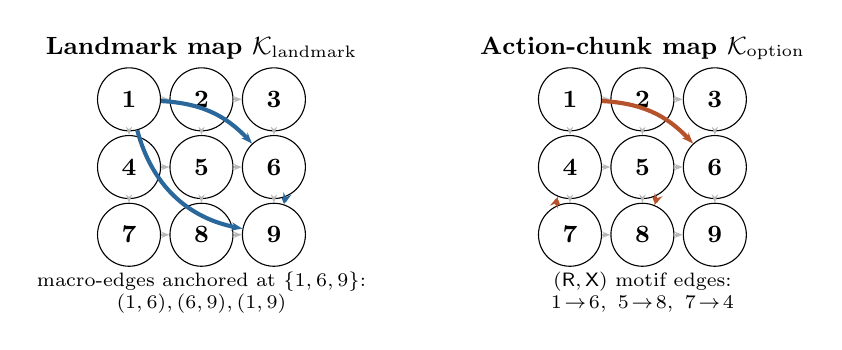
\begin{tikzpicture}[x=0.92cm,y=0.86cm]
% ---- left: landmark map ----
\begin{scope}
  \node[font=\bfseries\small] at (1,2.75) {Landmark map $\mathcal K_{\mathrm{landmark}}$};
  \foreach \n/\x/\y/\st in {1/0/2/L,2/1/2/N,3/2/2/N,4/0/1/N,5/1/1/N,6/2/1/L,7/0/0/N,8/1/0/N,9/2/0/L}{
    \ifx\st L \node[task landmark] (L\n) at (\x,\y) {\n};
    \else \node[task state] (L\n) at (\x,\y) {\n};\fi}
  \foreach \a/\b in {L1/L2,L2/L3,L4/L5,L5/L6,L7/L8,L8/L9,L1/L4,L4/L7,L2/L5,L5/L8,L3/L6,L6/L9}{
    \draw[gridedge] (\a)--(\b);}
  \draw[macroL] (L1) to[bend left=22] (L6);
  \draw[macroL] (L6) to[bend left=18] (L9);
  \draw[macroL] (L1) to[bend right=32] (L9);
  \node[font=\scriptsize,align=center] at (1,-0.85)
    {macro-edges anchored at $\{1,6,9\}$:\\ $(1,6),(6,9),(1,9)$};
\end{scope}
% ---- right: chunk map ----
\begin{scope}[xshift=5.6cm]
  \node[font=\bfseries\small] at (1,2.75) {Action-chunk map $\mathcal K_{\mathrm{option}}$};
  \foreach \n/\x/\y in {1/0/2,2/1/2,3/2/2,4/0/1,5/1/1,6/2/1,7/0/0,8/1/0,9/2/0}{
    \node[task state] (C\n) at (\x,\y) {\n};}
  \foreach \a/\b in {C1/C2,C2/C3,C4/C5,C5/C6,C7/C8,C8/C9,C1/C4,C4/C7,C2/C5,C5/C8,C3/C6,C6/C9}{
    \draw[gridedge] (\a)--(\b);}
  \draw[macroG] (C1) to[bend left=22] (C6);
  \draw[macroG] (C5) to[bend left=22] (C8);
  \draw[macroG] (C7) to[bend left=22] (C4);
  \node[font=\scriptsize,align=center] at (1,-0.85)
    {$(\mathsf R,\mathsf X)$ motif edges:\\ $1\!\to\!6,\ 5\!\to\!8,\ 7\!\to\!4$};
\end{scope}
\end{tikzpicture}
\caption{Induced cognitive maps. Both retain the primitive grid (grey). The landmark map
(blue) adds three hub-anchored macro-edges; the chunk map (orange) repeats the
$(\mathsf R,\mathsf X)$ macro-edge at every executable location. They overlap only at
$1\to6$.}
\label{fig:maps}
\end{figure}

\section{Can we recover them? System-identification questions and proposed tests}
\label{sec:recover}

This section states the questions and the tests; it does not run them. All inference uses
the synchronized structural EM of Analysis~7 (E-step over segmentations $Z_n$, M-step over
$\Theta_M$, outer structure search over $\mathcal R_M$ with a within-family BDeu proposal
diagnostic and a unified acceptance objective), and all contrasts are gated on simulation
recovery before any human interpretation.

\begin{description}[leftmargin=1.6em,style=nextline]
\item[Q1. Family recovery.] Given trajectories $\{\tau_n\}$ from this task set, can
structural EM recover the generating family (primitive / chunk / landmark)?
\emph{Test:} simulate each agent, fit all three families, report a model-confusion matrix;
success is near-diagonal mass at the planned trial counts. Predict that the
\emph{canonical-only} design is weakly identifiable (the twins alias) and that confusion
collapses once perturbation and novel-start trials are added.
\item[Q2. Structure recovery.] Does EM recover the correct discrete structure---
$\mathcal L=\{1,6,9\}$ with $\mathcal E^{\mathcal L}$ for the landmark agent, and
$\mathcal G\ni(\mathsf R,\mathsf X)$ for the chunk agent---rather than the decoy?
\emph{Test:} structure-recovery plots; report the false-positive rate for the centre-$5$
landmark and for spurious chunks, and check sensitivity over
$\alpha_{\mathrm{BD}}\in\{0.1,1,5,10\}$.
\item[Q3. Which data streams are necessary.] Are trajectories alone sufficient, or are
$D^{\mathrm{near}}$, $D^{\mathrm{chunk}}$, or perturbation trials required?
\emph{Test:} probe-stream ablation---recompute the confusion matrix and the held-out
trajectory-likelihood gap with streams added cumulatively; identify the minimal sufficient
set.
\item[Q4. Task-design levers.] Which trial types maximize separation?
\emph{Test:} compare designs that add (a) an express-edge block, (b) novel starts
converging on hub $6$, (c) probes at $5$ and $7$ that separate motif edges from anchors,
and (d) multiple-shortest-path trials ($\mu_{\mathrm{sp}}>1$) that elicit route
variability. Ask for the smallest trial subset that clears the recovery threshold.
\item[Q5. Identifiability boundary (the mimicry risk).] Can a chunk agent with tuned
execution noise and extra strings emulate the landmark agent's route flexibility well
enough to be unrecoverable from trajectories alone?
\emph{Test:} fit both and compare on held-out trajectory likelihood and on the approximate
family posterior $\widetilde p(M\mid D)$; check whether the structural prior (parsimony of a
single endpoint relation versus a proliferation of strings) and the perturbation trials
restore separation. A negative result here is informative: it would mandate the auxiliary
probes.
\item[Q6. Metrics and thresholds.] What counts as recovered?
\emph{Test:} report confusion-matrix diagonal mass, a structure-recovery score against the
true $(\mathcal L,\mathcal E^{\mathcal L})$ / $\mathcal G$, the held-out log-likelihood gap,
and the windowed structural-evidence trajectory
$L_n^{(M)}=\log p(D_{n-w+1:n}\mid M)-\log p(D_{n-w+1:n}\mid M_{\mathrm{primitive}})$,
with the window $w$ and the recovery threshold fixed during simulation before human data
are interpreted.
\end{description}

\section{Summary}

A landmark-option agent with the three optimal landmarks $\{1,6,9\}$ plans by selecting
endpoint-to-endpoint options at landmarks and realizing them with a target-directed
primitive kernel; on the express grid this yields the route $1\to2\to6\to9$ with flexible
realizations. Its closest action-chunk twin stores the single string $(\mathsf R,\mathsf X)$
and reproduces the same modal trajectory, but binds the segment to an action string rather
than an endpoint pair. The two agents are identical on the trained trial and differ
systematically off it: under express-block, novel-start, and at-$5$/$7$ probes, under route
variability, and in their nearness and chunk judgments; and their cognitive maps place
macro-edges at the anchors $\{1,6,9\}$ versus at the motif locations $\{1\!\to\!6,5\!\to\!8,
7\!\to\!4\}$. Whether the planned behavioural design can separate them is an empirical
question for simulation-gated structural-EM recovery, posed above as Q1--Q6.

\end{document}
